\documentclass{ximera}
\input{../preamble.tex}

\author{Robert Kenney \and Paul Zachlin \and Nicholas Shay}
\title{An Introduction to Control Charts} \license{CC BY-NC-SA 4.0}
\begin{document}

\begin{abstract}
We explore an application of concepts related to the normal distribution to manufacturing.
\end{abstract}
\maketitle

\begin{onlineOnly}
\section*{An Introduction to Control Charts}
\end{onlineOnly}

\subsection*{Out of Control}

\begin{exploration}\label{exp:OJ}
  A machine at a juice factory is set to fill juice bottles with 300 ml of juice.  If the process is operating normally, the mean amount of juice per bottle is historically known to be normally distributed with $\mu=300$ ml, and standard deviation of $\sigma=2$ ml. To check how well the process is running the factory routinely samples their output to avoid under-filling or over-filling the bottles.  Six samples of size $n=4$ are shown below.

\begin{center}
        \begin{tikzpicture}
\node[inner sep=0pt, anchor=base] (p1) at (0,0)
  {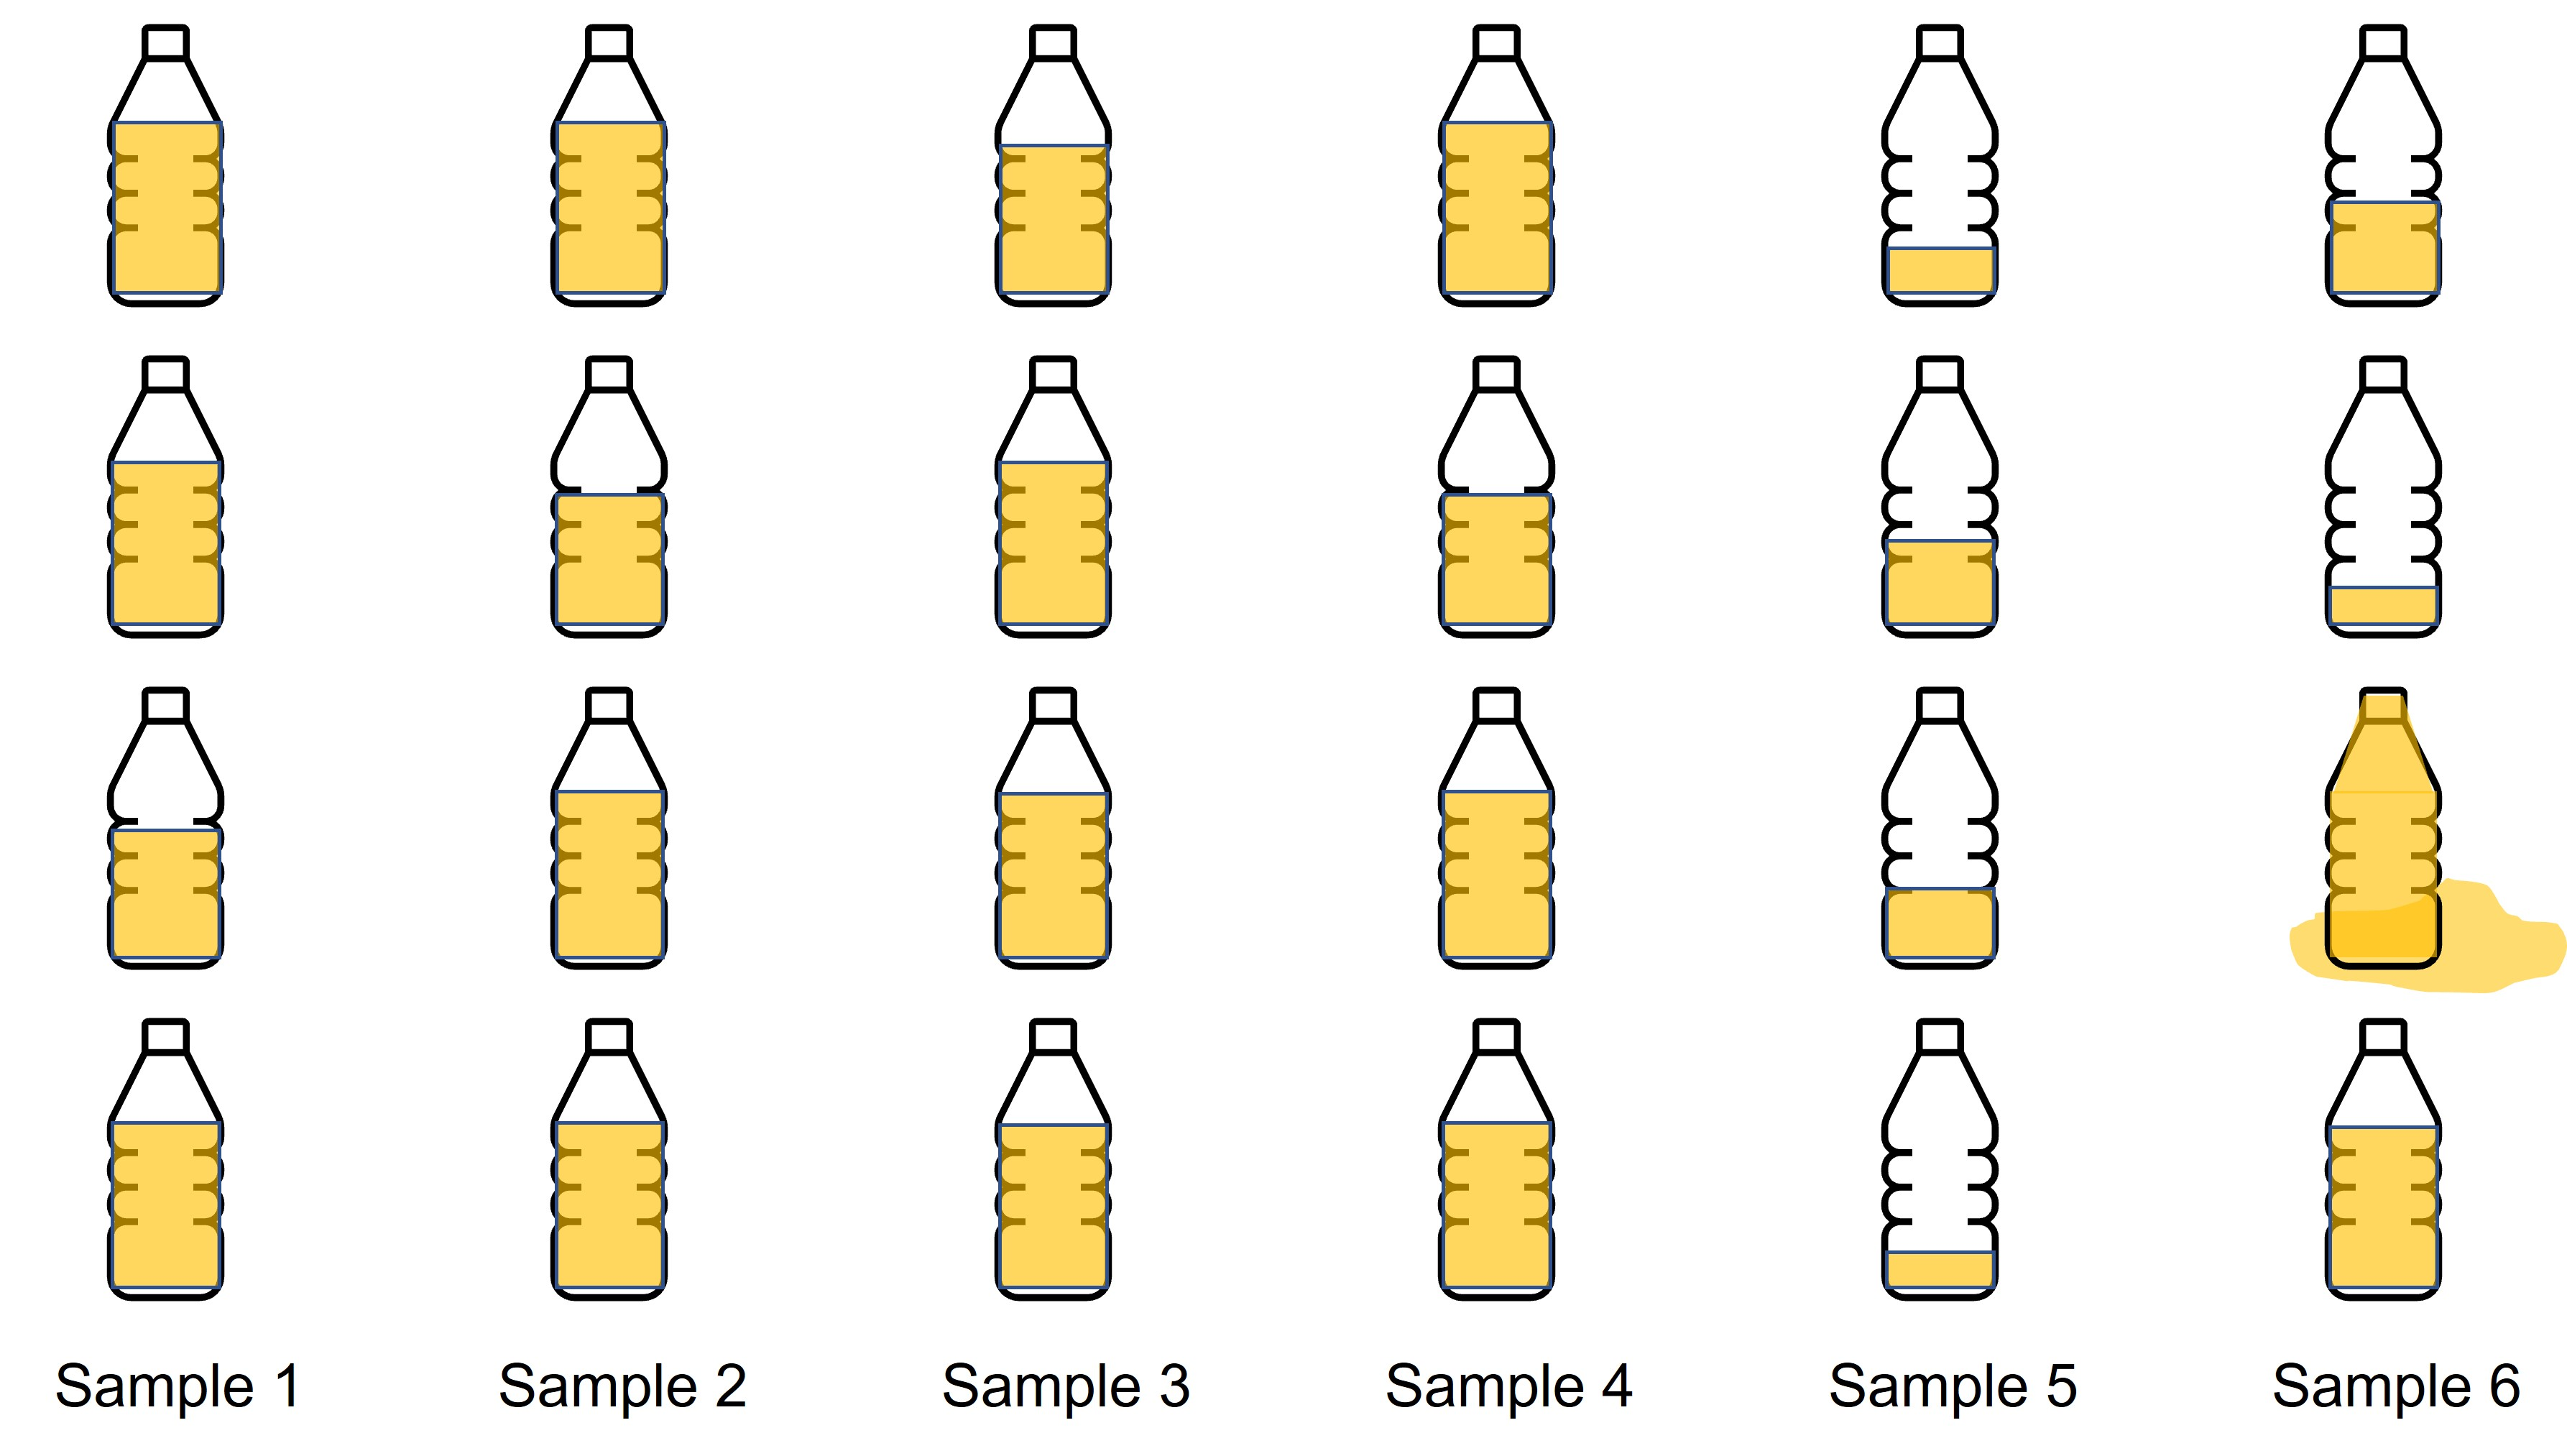
\includegraphics[height=60mm]{bottlesOJ.jpg}};
           \end{tikzpicture}
      \end{center}

Variability is a normal part of any manufacturing process.  The first four samples are depicted to represent amounts close to 300 ml, and a reasonable amount of variation.  Samples 5 and 6 are sketched to illustrate a process gone wrong.  If you compare samples 5 and 6 carefully, you will see that each sample points to a different kind of problem with the process.

Samples are collected to gauge the current state of the process.  What does sample 5 indicate about the process?

\begin{multipleChoice}
\choice{The process is no longer consistent.  Standard deviation is too high.}
\choice[correct]{The mean is much less than 300 ml.}
\choice{The mean is much greater than 300 ml.}
\end{multipleChoice}

What does sample 6 indicate about the process?

\begin{multipleChoice}
\choice[correct]{The process is no longer consistent.  Standard deviation is too high.}
\choice{The mean is much less than 300 ml.}
\choice{The mean is much greater than 300 ml.}
\end{multipleChoice}
 
\end{exploration}

Variability is a natural part of any manufacturing process.  
\emph{Natural cause variation} or \emph{common cause variation} is a result interactions between people, equipment, method, material, and environment.  This variation is a result of the whole system, not assignable to a particular incident or part.  It may be reduced ONLY by changing the system.

\emph{Assignable cause variation} or \emph{special cause variation} is a result of a particular, assignable incident or process part. This type of variation may be easy to identify and fix with a ``tweak".

\emph{in-control process} 

\emph{out-of-control process} 

Samples 5 and 6 suggest that the process is out of control, statistical analysis will help us determine whether or not this is the case. 

\subsection*{Something significant...}
Let's take a look at the data corresponding to the graphic in Exploration \ref{exp:OJ}.  In the table below, individual volumes are listed for each sample along with numerical summaries.  You are familiar with sample mean ($\bar{x}$) and sample standard deviation ($s$).  You may or may not have seen the  \emph{range}, denoted by $R$.  The range, just like standard deviation, is a measure of spread of data.  It is given by the difference between the largest and the smallest values in the sample.  
$$R=\text{largest data point}-\text{smallest data point}$$

Both range ($R$) and sample standard deviation ($s$) can be used to estimate population standard deviation ($\sigma$), but because the range takes into account only the two extreme values in the sample, it fails to capture the nuances of the spread, like standard deviation does.  For small samples ($n\leq 6$), either $R$ or $s$ can be used to estimate $\sigma$ with approximately the same efficiency.  As a result, when dealing with small samples, range is typically preferred over standard deviation due to ease of computations. (Montgomery)

Compute $R$ for samples 3 and 6 and enter your answers in the cells provided.

\begin{center}
\begin{tabular}{|c|c|c|c|c|c|c|}
& Sample 1 & Sample 2 & Sample 3 & Sample 4 & Sample 5 & Sample 6  \\
 \hline
 \hline
   & & & & & &\\
 &300 & 299 & 298 & 302 & 295 &296 \\
  & & & & & &\\
%  \hline
  & & & & & &\\
 &300 & 297 & 299 & 298 & 296 & 305\\
  & & & & & &\\
% \hline
 & & & & & &\\
 &299 & 299 & 300 & 300 & 297 & 299 \\
  & & & & & &\\
% \hline
  & & & & & &\\
 &302 & 301  & 301 & 300 &297 & 298 \\
  & & & & & &\\
 \hline
 \hline
  & & & & & &\\
 $\bar{x}=$ & 300.25 & 299  & 299.5 & 300 & 296.25 & 299.5 \\
  & & & & & &\\
  \hline
  & & & & & &\\
 $s=$ & 1.26 & 1.63  & 1.29 & 1.63 & 0.96 & 3.87 \\
  & & & & & &\\
 \hline
   & & & & & &\\
 $R=$ & 3 & 4  & $\answer{3}$ & 4 & 2 & $\answer{9}$ \\
  & & & & & &\\
 \hline
\end{tabular}
\end{center}

Observe that sample mean for sample 5 is considerably lower than the other sample means, and also lower than the presumed population mean ($\mu=300$).  Observe also that the volumes in sample 6 are more spread out than the volumes in the other samples, as indicated by the magnitudes of $R$ and $s$.  Is this part of the natural variation inherent in any manufacturing process, or is this an indication that the process is no longer in control?  The following questions will guide you to the answer.

\begin{question}\label{quest:popBellCurve}
Recall that this population is normally distributed with $\mu=300$ ml, and $\sigma=2$ ml.  

Select the most appropriate graph to represent the historically established population distribution.

\begin{hint}
    Use the Empirical Rule.
\end{hint}

\begin{multipleChoice}
 \choice{Impossible to determine from the information given. }
\choice[correct]{
      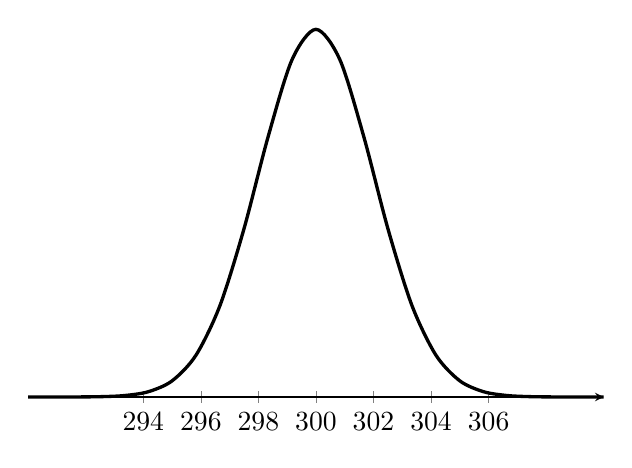
\begin{tikzpicture}
        \begin{axis}[
          domain=290:310,
          xmin=290, xmax=310,
          ymin=-0.01, ymax=0.25,
          width=3.5in,
          xtick={294,296, 298,300,302,304,306},
            xticklabels={$294$,$296$,$298$,$300$, $302$,$304$,$306$},
           % ytick style={draw=none},
            %yticklabels={},
            axis x line=center,
            axis y line=none,
          %axis lines =middle, xlabel={}, ylabel={},
          %every axis y label/.style={at=(current axis.above origin),anchor=south},
           every axis x label/.style={at=(current axis.right of origin),anchor=west},
          ]
      \addplot [very thick,  smooth] {(e^(-0.5*((x-300)/2)^2))/(((2*pi)^0.5)*2)};
      %    \node at (axis cs:320, 0.025 ) [anchor=west] {$A$};
          \end{axis}
        \end{tikzpicture}
}
\choice{
       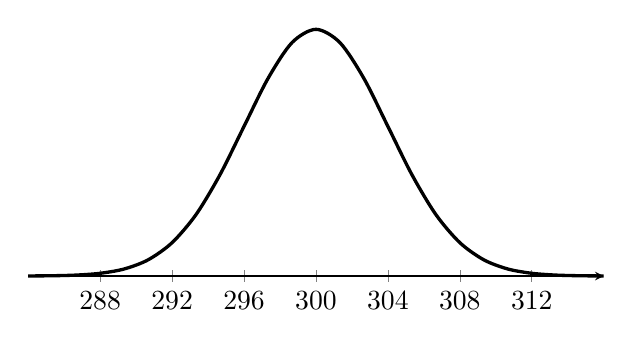
\begin{tikzpicture}
        \begin{axis}[
          domain=290:310,
          xmin=290, xmax=310,
          ymin=-0.01, ymax=0.3,
          width=3.5in,
          xtick={292.5, 295, 297.5,300,302.5,305, 307.5},
            xticklabels={$288$,$292$,$296$,$300$, $304$,$308$,$312$},
           % ytick style={draw=none},
            %yticklabels={},
            axis x line=center,
            axis y line=none,
          %axis lines =middle, xlabel={}, ylabel={},
          %every axis y label/.style={at=(current axis.above origin),anchor=south},
           every axis x label/.style={at=(current axis.right of origin),anchor=west},
          ]
      \addplot [very thick,  smooth] {(e^(-0.5*((x-300)/2.5)^2))/(((2*pi)^0.5)*2.5)};
          %\node at (axis cs:395, 0.25 ) [anchor=west] {$B$};
          \end{axis}
        \end{tikzpicture}
        }
        \choice{
        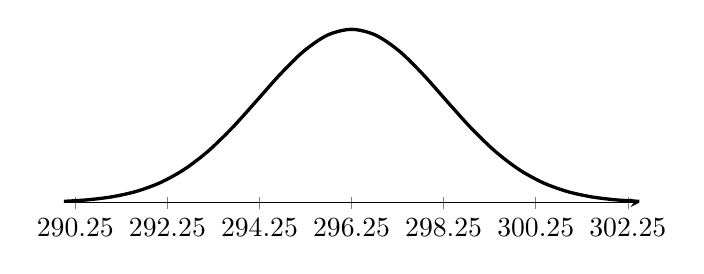
\begin{tikzpicture}
        \begin{axis}[
          domain=290:302.5,
          xmin=290, xmax=302.5,
          ymin=-0.01, ymax=0.1,
          width=3.5in,
          xtick={290.25,292.25,294.25,296.25, 298.25,300.25,302.25},
            xticklabels={$290.25$,$292.25$,$294.25$,$296.25$, $298.25$,$300.25$,$302.25$},
           % ytick style={draw=none},
            %yticklabels={},
            axis x line=center,
            axis y line=none,
          %axis lines =middle, xlabel={}, ylabel={},
          %every axis y label/.style={at=(current axis.above origin),anchor=south},
           every axis x label/.style={at=(current axis.right of origin),anchor=west},
          ]
      \addplot [very thick,  smooth] {(e^((-(x-296.25)^2)/(2*2^2)))/(2*pi*2^2)};
         % \node at (axis cs:405, 0.025 ) [anchor=west] {$C$};
          \end{axis}
        \end{tikzpicture}
        }
\end{multipleChoice}


\end{question}

\begin{question}\label{quest:samplingDist}
    Now we turn our attention to the distribution of sample means, also known as sampling distribution.  Given that the population is normally distributed with $\mu=300$ ml, and $\sigma=2$ ml, find the mean and standard deviation for the sampling distribution for samples of size 4 ($n=4$).

    $$\mu_{\bar{X}}=\answer{300},\quad \sigma_{\bar{X}}=\answer{1}$$

\begin{hint}
    Use the Central Limit Theorem.
\end{hint}    

Select the most appropriate graph to represent the sampling distribution for $n=4$.

\begin{multipleChoice}
 \choice{Impossible to determine from the information given. }
\choice{
      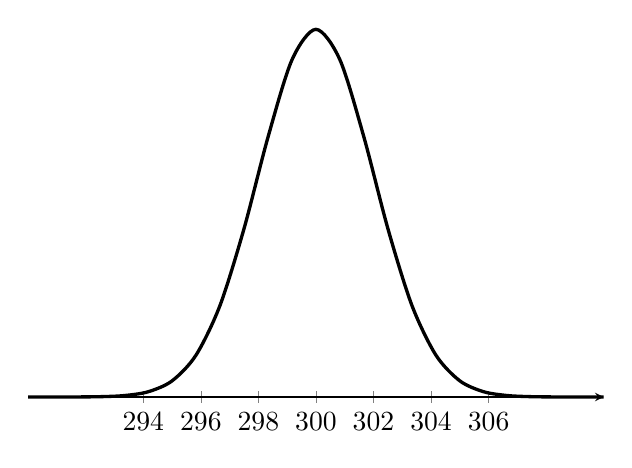
\begin{tikzpicture}
        \begin{axis}[
          domain=290:310,
          xmin=290, xmax=310,
          ymin=-0.01, ymax=0.25,
          width=3.5in,
          xtick={294,296, 298,300,302,304,306},
            xticklabels={$294$,$296$,$298$,$300$, $302$,$304$,$306$},
           % ytick style={draw=none},
            %yticklabels={},
            axis x line=center,
            axis y line=none,
          %axis lines =middle, xlabel={}, ylabel={},
          %every axis y label/.style={at=(current axis.above origin),anchor=south},
           every axis x label/.style={at=(current axis.right of origin),anchor=west},
          ]
      \addplot [very thick,  smooth] {(e^(-0.5*((x-300)/2)^2))/(((2*pi)^0.5)*2)};
      %    \node at (axis cs:320, 0.025 ) [anchor=west] {$A$};
          \end{axis}
        \end{tikzpicture}
}
\choice{
       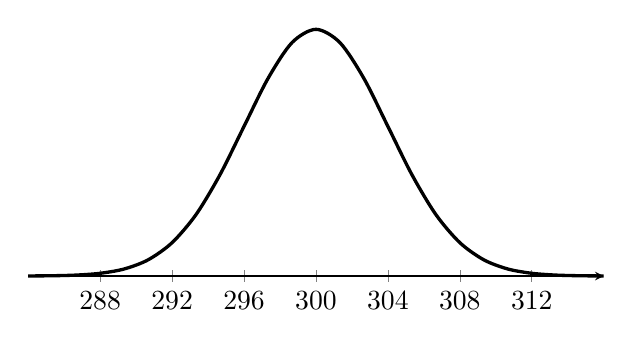
\begin{tikzpicture}
        \begin{axis}[
          domain=290:310,
          xmin=290, xmax=310,
          ymin=-0.01, ymax=0.3,
          width=3.5in,
          xtick={292.5, 295, 297.5,300,302.5,305, 307.5},
            xticklabels={$288$,$292$,$296$,$300$, $304$,$308$,$312$},
           % ytick style={draw=none},
            %yticklabels={},
            axis x line=center,
            axis y line=none,
          %axis lines =middle, xlabel={}, ylabel={},
          %every axis y label/.style={at=(current axis.above origin),anchor=south},
           every axis x label/.style={at=(current axis.right of origin),anchor=west},
          ]
      \addplot [very thick,  smooth] {(e^(-0.5*((x-300)/2.5)^2))/(((2*pi)^0.5)*2.5)};
          %\node at (axis cs:395, 0.25 ) [anchor=west] {$B$};
          \end{axis}
        \end{tikzpicture}
        }
        \choice[correct]{
        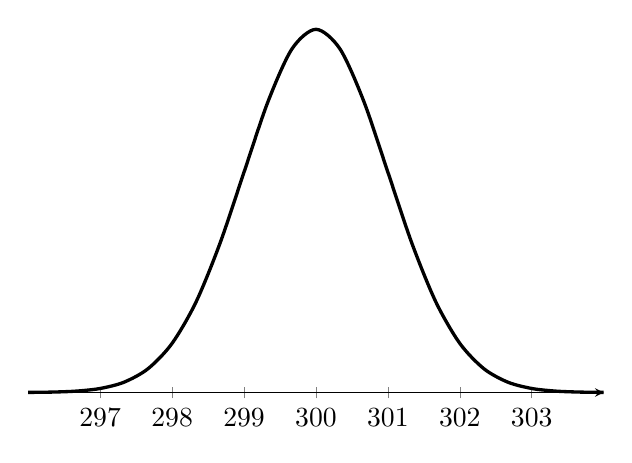
\begin{tikzpicture}
        \begin{axis}[
          domain=296:304,
          xmin=296, xmax=304,
          ymin=-0.01, ymax=0.2,
          width=3.5in,
          xtick={297,298,299,300, 301,302,303},
          %  xticklabels={297,298,299,300, 301,302,303},
           % ytick style={draw=none},
            %yticklabels={},
            axis x line=center,
            axis y line=none,
          %axis lines =middle, xlabel={}, ylabel={},
          %every axis y label/.style={at=(current axis.above origin),anchor=south},
           every axis x label/.style={at=(current axis.right of origin),anchor=west},
          ]
      \addplot [very thick,  smooth] {(e^((-(x-300)^2)/(2*1^2)))/(2*pi*1^2)};
         % \node at (axis cs:405, 0.025 ) [anchor=west] {$C$};
          \end{axis}
        \end{tikzpicture}
        }
     \end{multipleChoice}
    
\end{question}

Now that we know what the sampling distribution should look like, let's take a look at our samples.  Advance the slider to see where each sample mean falls within this distribution.  

\begin{onlineOnly}
\begin{center}
\geogebra{uy3fusxy}{950}{650}
\end{center}
\end{onlineOnly}

Observe that all sample means, with the exception of sample 5, are located in the green zone near the center of the graph.  The green zone, also known as Zone 1, is located between $\mu -\sigma$ and $\mu+\sigma$.  From the Empirical Rule, we know that approximately $68\%$ of data are located in this zone. 

Sample 5 mean is located more than three standard deviations away from the mean.  From the Empirical Rule, we know that approximately $99.7\%$ of data are located within three standard deviations from the mean.  Therefore, the probability of sample 5, or a more extreme sample, occurring is very near zero.  What can this tell us?

\begin{idea}
IF the process is under control ($\mu=300, \sigma=1$), then there is essentially ZERO chance of us getting a sample such as sample 5, or a more extreme sample.  Because such a sample DID occur, we conclude that the process must be out of control, and must be paused.
\end{idea}

\subsubsection*{Turning the normal distribution on its side}

To monitor a process over time, we will mark times (or sample numbers) along the horizontal axis, and the relevant sample statistic on the vertical axis.  Just like we marked the green, yellow and the red zones under the bell curve in the diagram above, we will mark green, yellow and red zones (Zones 1, 2, 3) to help us identify the zone where each sample mean falls.  We can even mentally add a bell curve to help us visualize the situation, as shown for sample 1.

\begin{onlineOnly}
\begin{center}
\geogebra{uhdwnkgs}{950}{650}
\end{center}
\end{onlineOnly}

The diagram above is an example of a \emph{Control Chart}.  Control charts are used by technicians and engineers supervising manufacturing processes to track sample means and spread in order to quickly detect a process no longer in control.  There are several types of control charts.  In the next section we will examine two most commonly used types.

\subsection*{Control Charts}

To make sure that a process is in control, it is essential to monitor variability as well as means.  In the previous section, we presented a control chart for sample means.  This kind of chart is called an \emph{x-bar chart}.  To monitor variability, either range ($R$) or sample standard deviation ($s$) can be used.  As discussed earlier, $R$ is much easier to compute than $s$, and produces similar results for small samples ($n\leq 6$).  As a result, \emph{R-charts}, which monitor the range, are used more often than \emph{s-charts}.

Let's return to our juice bottle example to examine what the x-bar chart and the R-chart tell us when taken together.  The following charts were generated in RStudio using the qcc package.

\begin{center}
         \begin{tikzpicture}
 \node[inner sep=0pt, anchor=base] (p1) at (0,0)
   {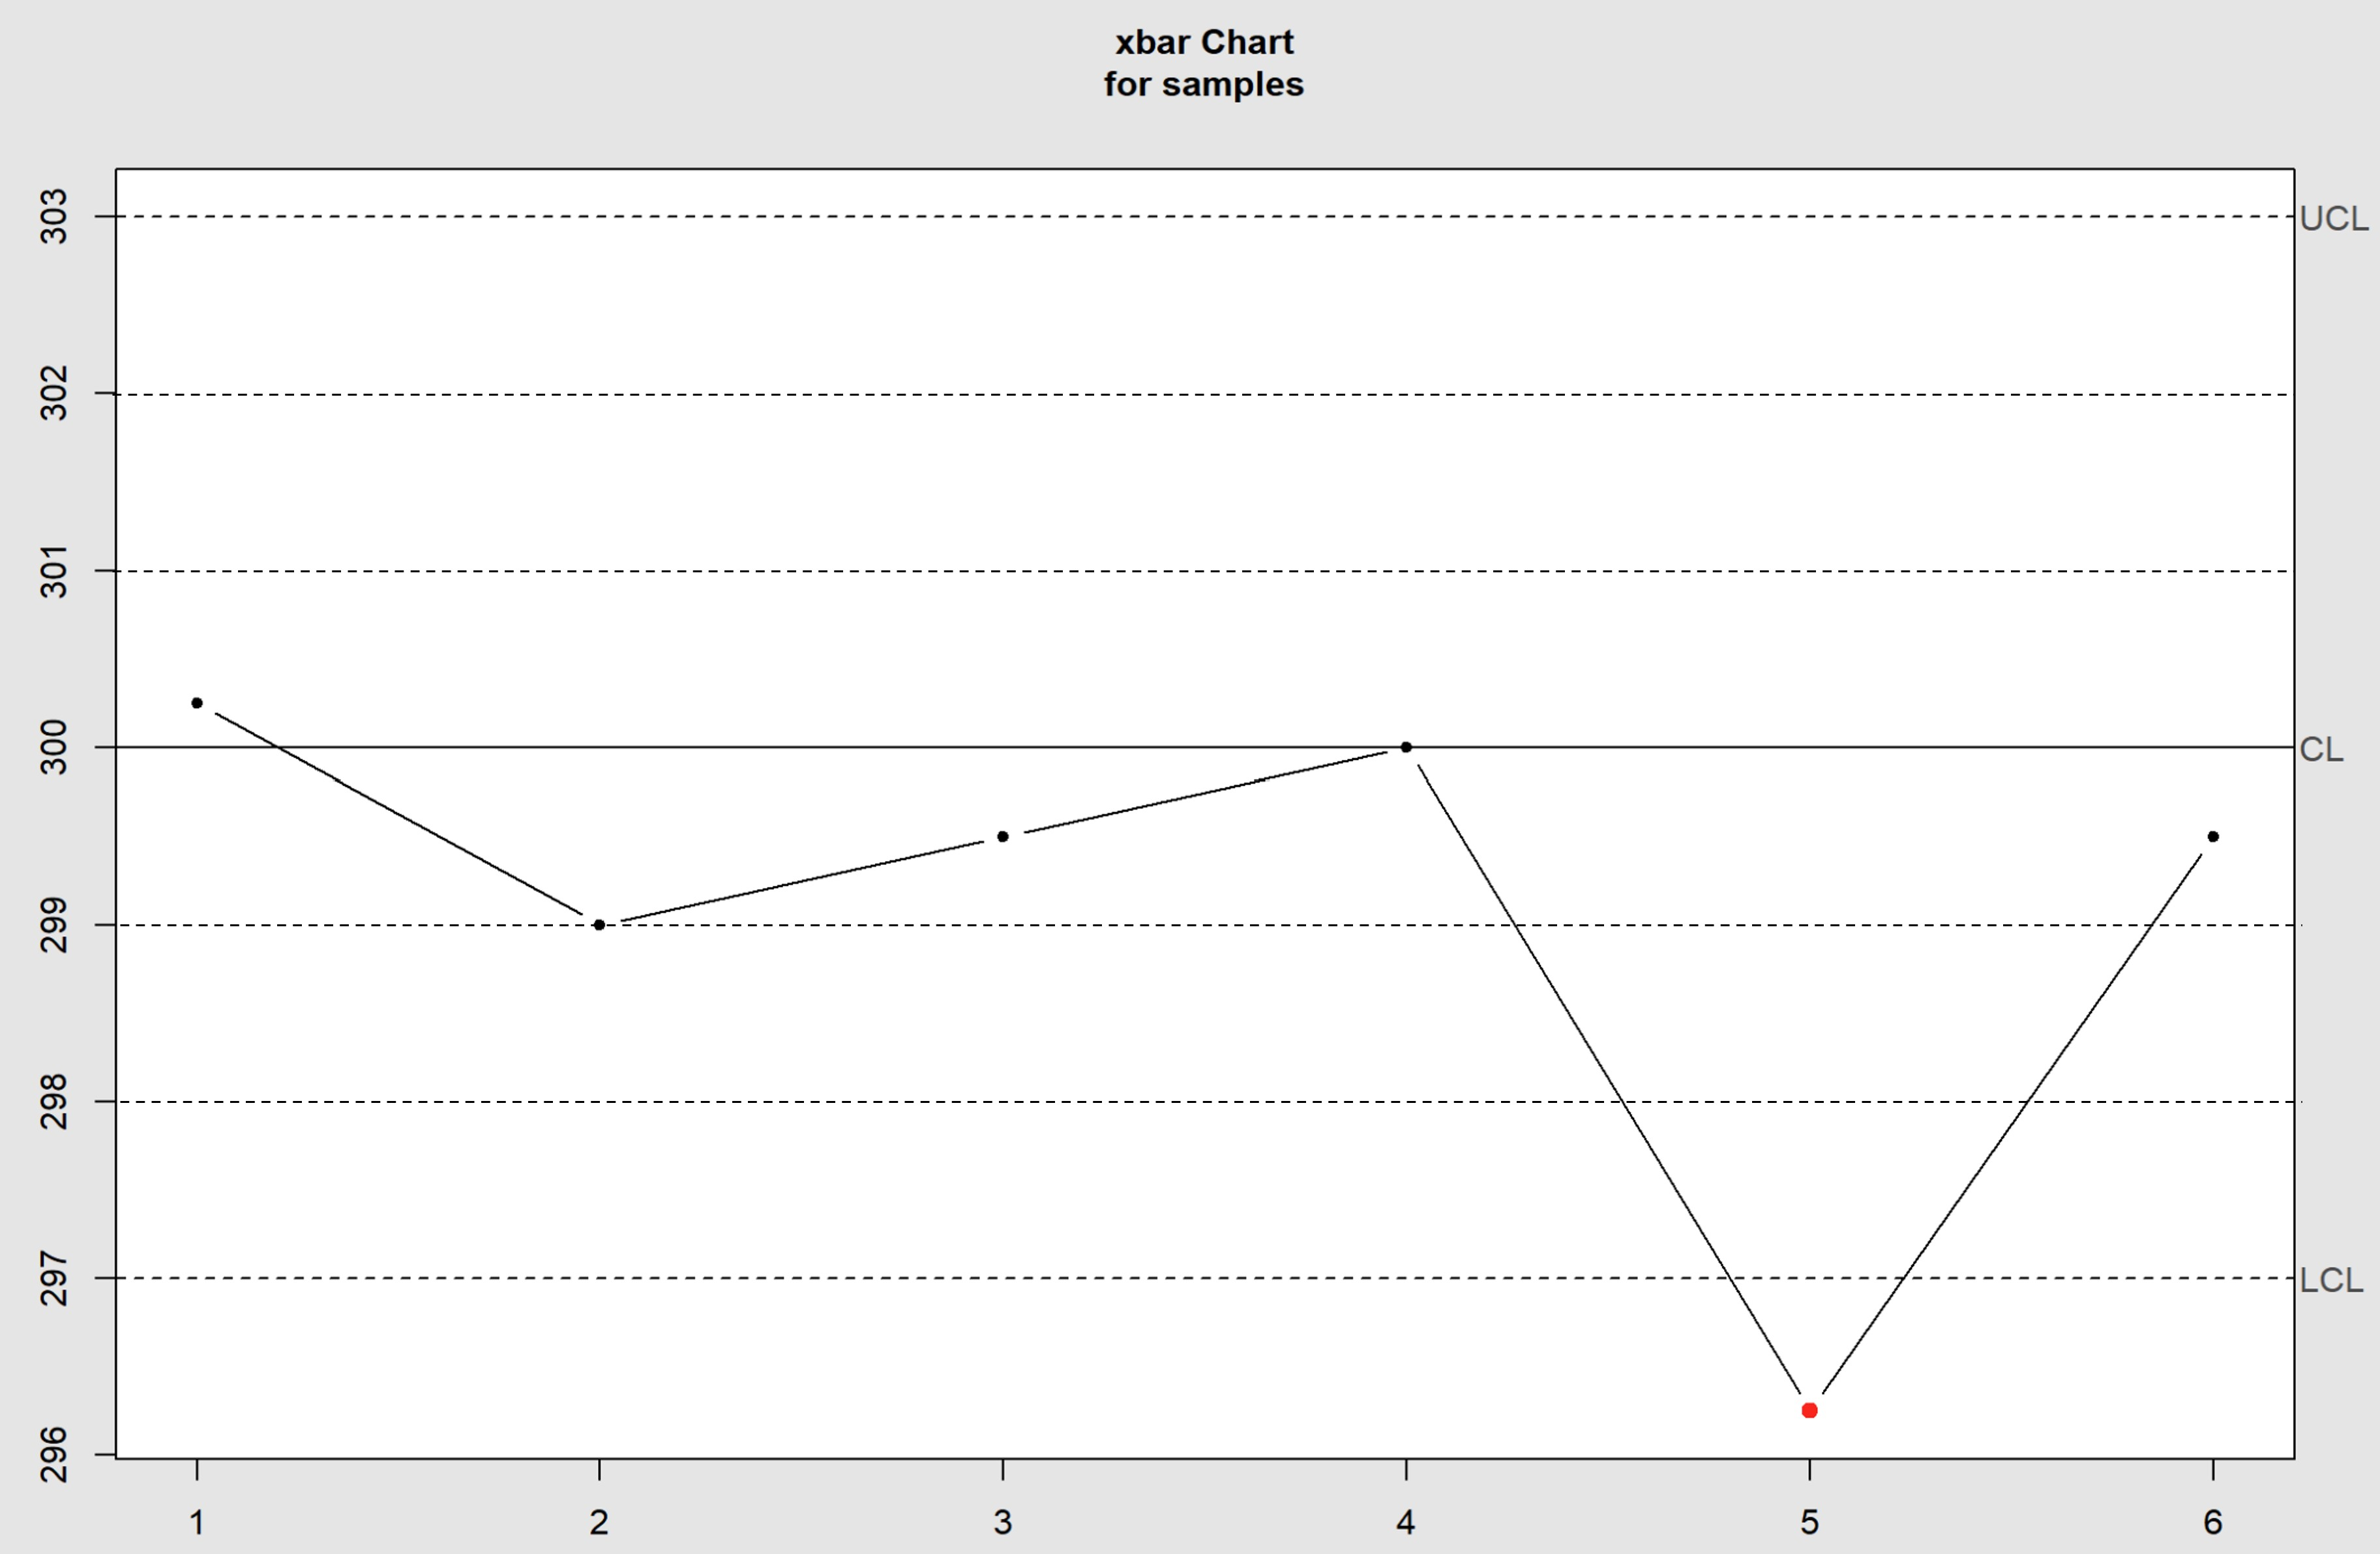
\includegraphics[height=100mm]{xBarChart.jpg}};
   \node[inner sep=0pt, anchor=base] (p2) at (16,0)
   {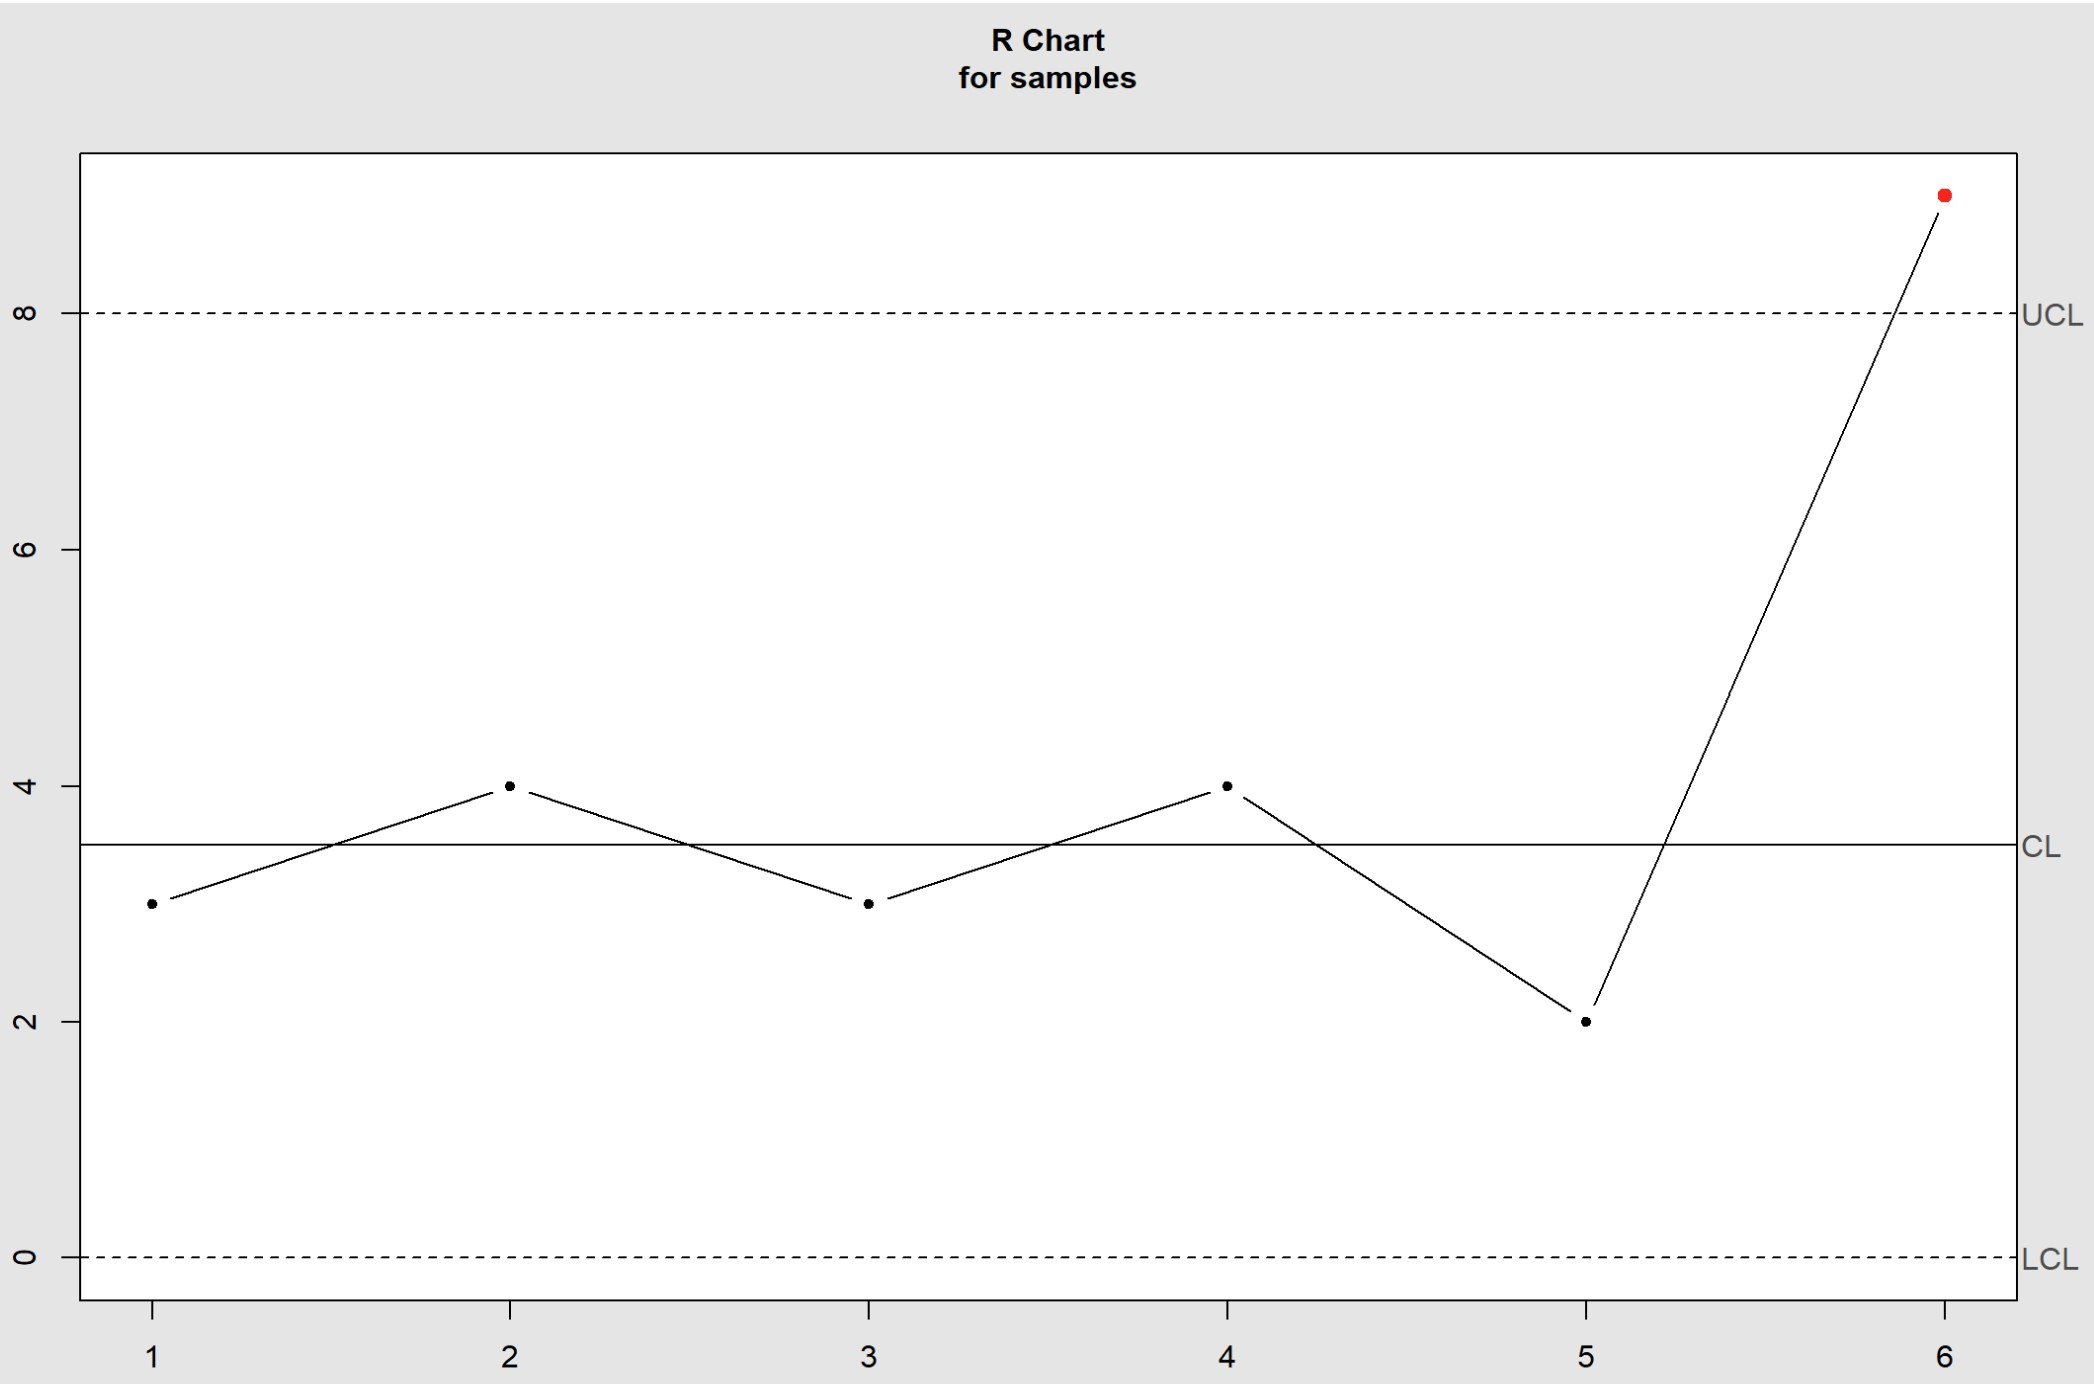
\includegraphics[height=100mm]{RChart.jpg}};
            \end{tikzpicture}
       \end{center}

This example highlights the reason why x-bar charts and R-charts should be used together.  The x-bar chart was sufficient to spot the problem with sample 5.  The problem with sample 6, however, would have been missed if we had used the x-bar chart alone. 




\section*{Rules}
Write out Whatever rules we decide to use.  

This is where I think my example from the next section would fit to prepare students for the case study.



\section*{Practice Problems}

\section*{References}

Montgomery, D. C. (2009). Statistical quality control: A modern introduction (6th ed.). Wiley.

\end{document} 